
    \newgeometry{top=1.5cm,bottom=1.5cm,left=1.5cm,right=1.5cm}
    \begin{landscape}
        \footnotesize
    \begin{figure}
        \thispagestyle{empty}
        \begin{subfigure}[t]{0.3\textwidth}\vskip 0pt
            \centering
            \begin{subfigure}[t]{\textwidth}\vskip 0pt
                \centering
                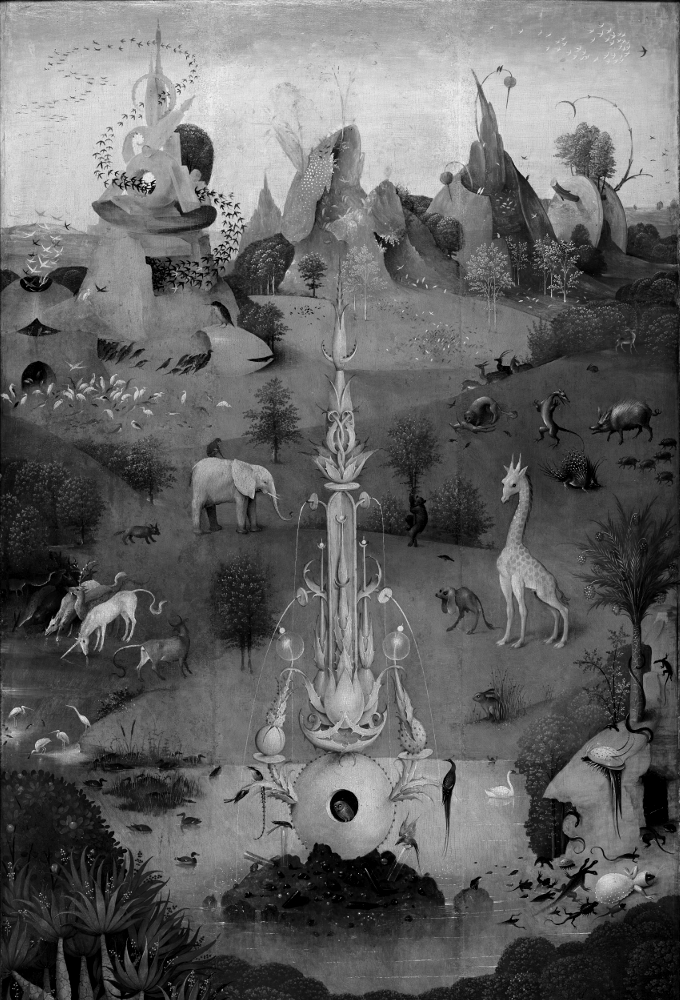
\includegraphics[width=\textwidth]{images/A1.png}
                \caption{Une première perspective marquée et s'étendant au loin. Ici, l'auditeur peut explorer une ménagerie positionnée en trois dimensions, ainsi que des sons doux émanant de la structure centrale.}
                \label{fig.a1}
            \end{subfigure}~\\       
            \begin{subfigure}[t]{\textwidth}\vskip 0pt
                \centering
                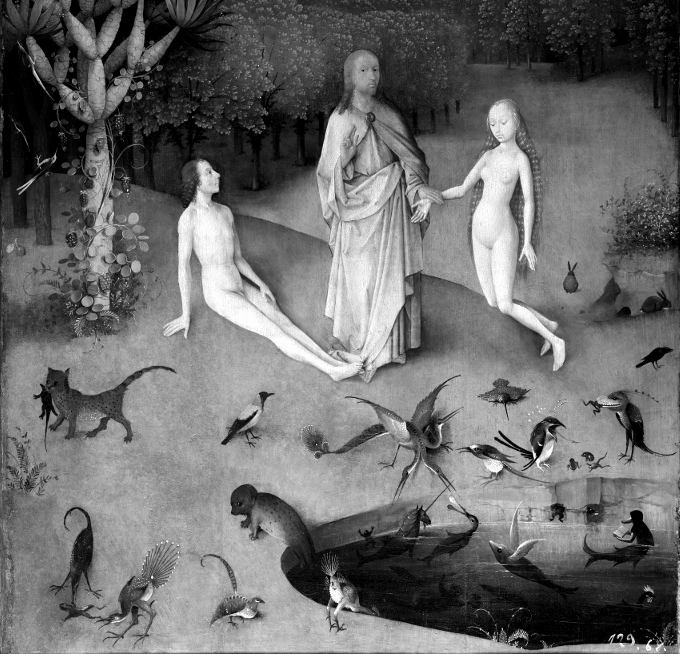
\includegraphics[width=\textwidth]{images/A2.png}
                \caption{Une scène faisant référence à la Genèse. Plusieurs scénarios sont possibles en fonction de l'ordre dans lequel les personnages sont actionnés.}
                \label{fig.a2}
            \end{subfigure}   
            \label{fig.a}
        \end{subfigure}\hspace{1cm}
        \begin{subfigure}[t]{0.7\textwidth}\vskip 0pt
            \centering
            \begin{subfigure}[t]{\textwidth}\vskip 0pt
                \centering
                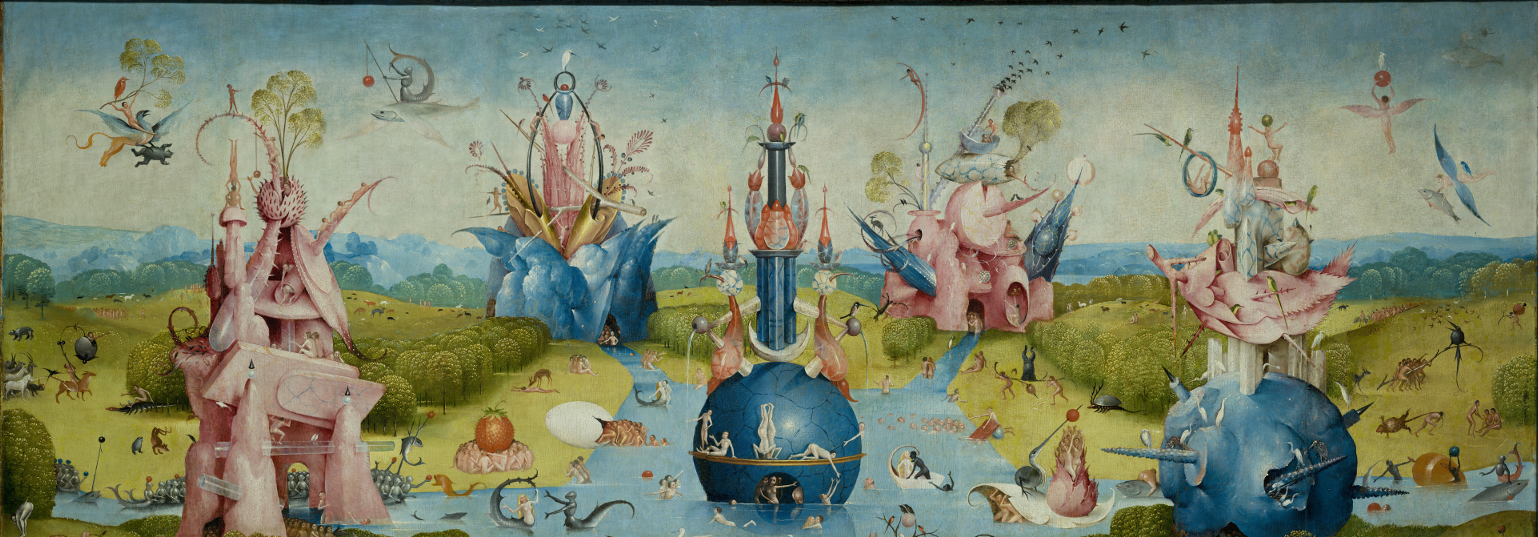
\includegraphics[width=\textwidth]{images/B1.png}
                \label{fig.b1}
                \caption{Les cinq structures font office d'instrument de musique spatialisé : chacun produira un son à une hauteur différente. Lorsque le premier est activé, des effets commencent à s'appliquer sur le son.}
            \end{subfigure}~\\           
            \begin{subfigure}[t]{\textwidth}\vskip 0pt
                \centering
                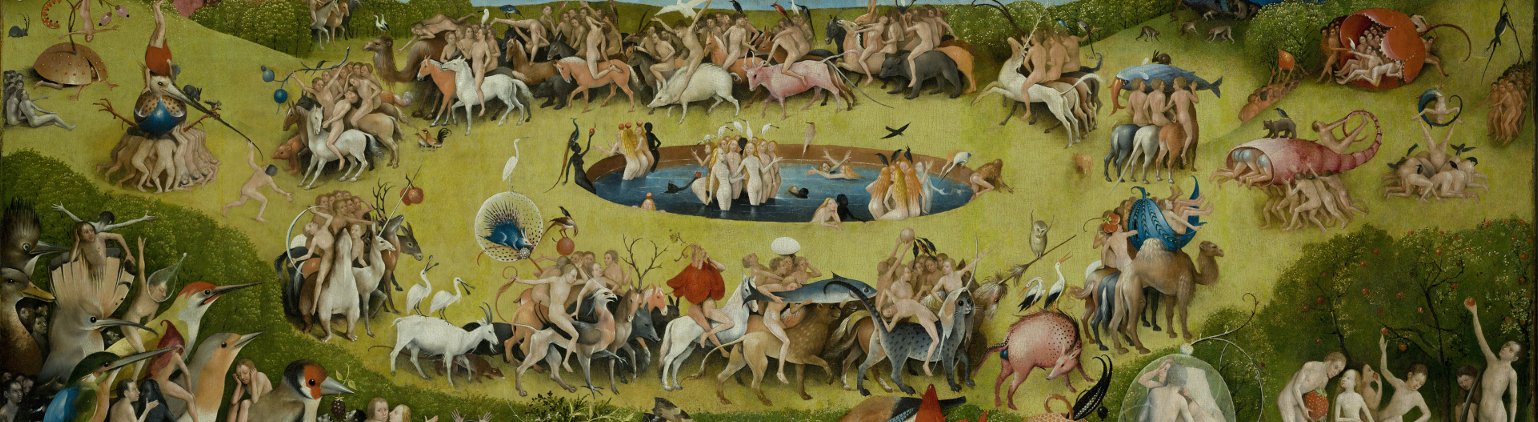
\includegraphics[width=\textwidth]{images/B2.png}
                \caption{Il est possible d'explorer cette scène en naviguant dans son espace; le mouvement invite à l'utilisation de trajectoires spatialisées.}
                \label{fig.b2}
            \end{subfigure}~\\          
            \begin{subfigure}[t]{\textwidth}\vskip 0pt
                \centering
                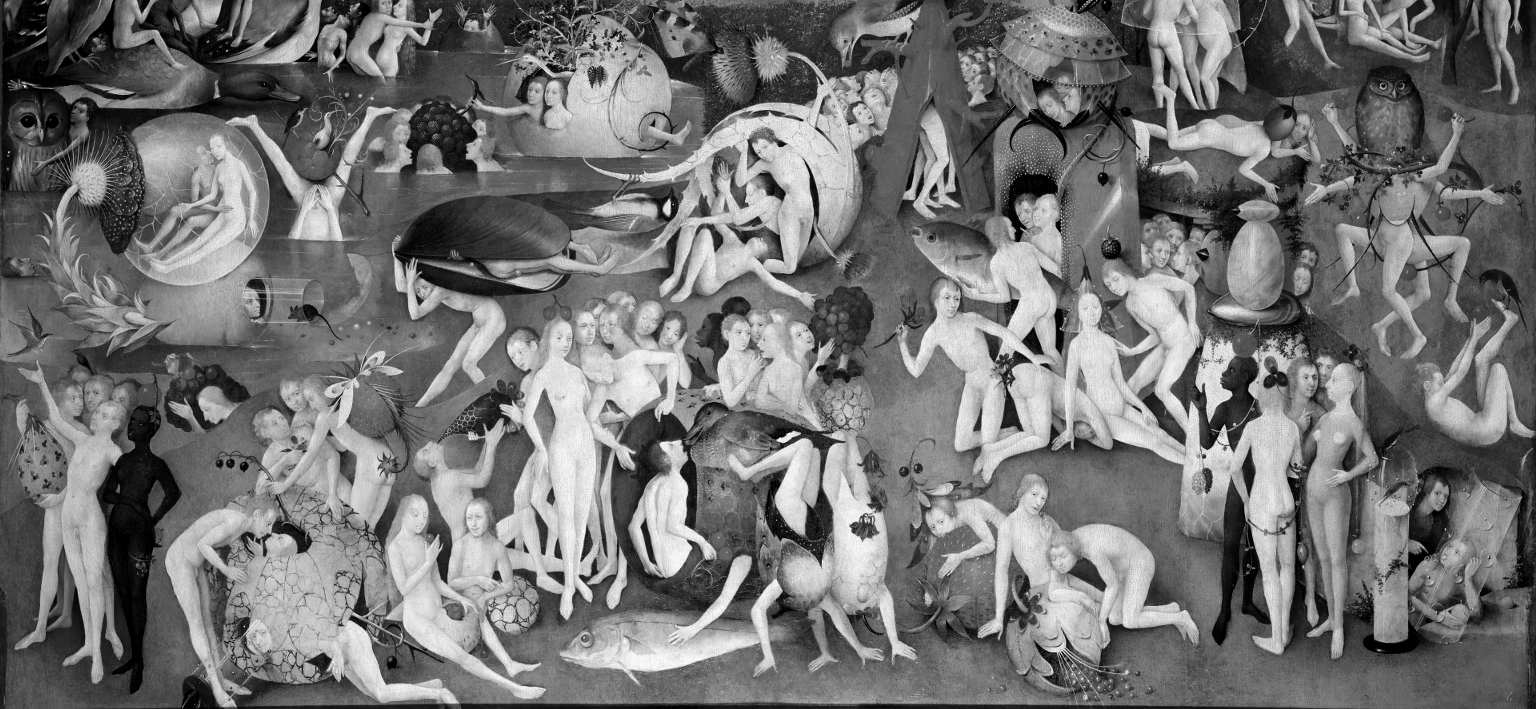
\includegraphics[width=\textwidth]{images/B3.png}
                \caption{Dans cette partie, des acteurs se déplacent en permanence; interagir avec certains d'entre eux aura des effets sur une trame globale pour cette scène, ainsi que pour l'ensemble du panneau.}
                \label{fig.b3}
            \end{subfigure}  
            \label{fig.b}
        \end{subfigure}\hspace{1cm}
        \begin{subfigure}[t]{0.3\textwidth}\vskip 0pt
            \centering
        \begin{subfigure}[t]{\textwidth}\vskip 0pt
            \centering
            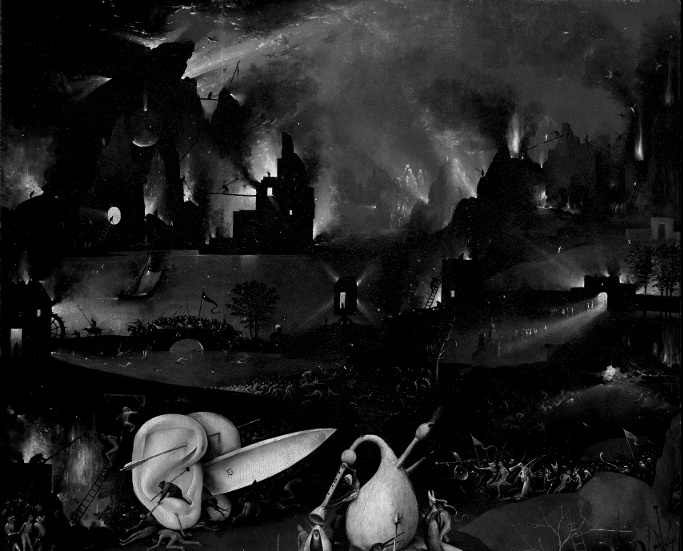
\includegraphics[width=\textwidth]{images/C1.png}
            \caption{L'enfer : des crépitements et sons discordants peuplent cette scène.}
            \label{fig.c1}
        \end{subfigure}~\\
        \begin{subfigure}[t]{\textwidth}\vskip 0pt
            \centering
            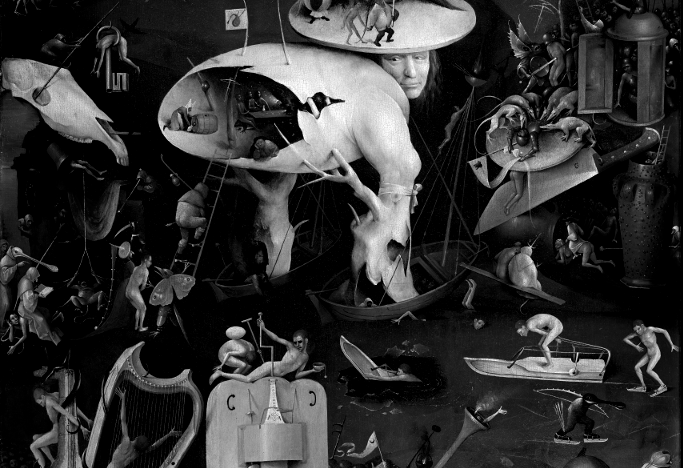
\includegraphics[width=\textwidth]{images/C2.png}
            \caption{Les personnages de cette scène vont peu à peu s'énerver au fil des interactions qu'a le public.}
            \label{fig.c2}
        \end{subfigure}~\\
        \begin{subfigure}[t]{\textwidth}\vskip 0pt
            \centering
            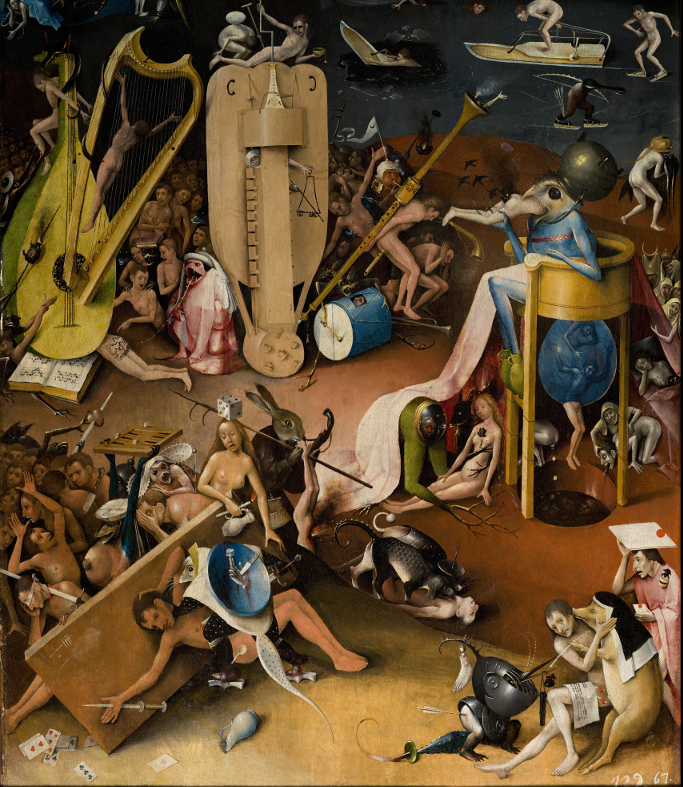
\includegraphics[width=\textwidth]{images/C3.png}
            \caption{Cette scène permet une interaction musicale avec les instruments, par le biais d'un moteur de synthèse granulaire.}
            \label{fig.C3}
        \end{subfigure}
        \end{subfigure}
        
        \caption{Description du tableau et séparation en plans}
        \label{fig.plans}
        
    \end{figure}
    \end{landscape}
    \restoregeometry